\label{sec::7_ah}
To close the control loop and to steer the robot towards desired goals, whilst avoiding obstacles, requires some high-level command that arises from visual feedback. As discussed in section \ref{sec::1_in} - Introduction, there are several ways to achieve this, among them human users. Of particular interest to us are novel methods that evolved from the toolbox of machine learning techniques, as they decrease the computational cost into nonexistence. Let alone this fact enables us to run them onboard on lightweight hardware with low energy usage, which is critical in the domain of humanoid robots. Center to these new methods will be neural nets that we will train on solving the task of autonomous navigation in two different ways. One of which clones the behavior of a human user (sec. \ref{sec::51_bc}), whereas the second presented method (sec. \ref{sec::42_rl}) explores policies and tries to find solutions on its own.
\begin{figure}[h!]
	\centering
	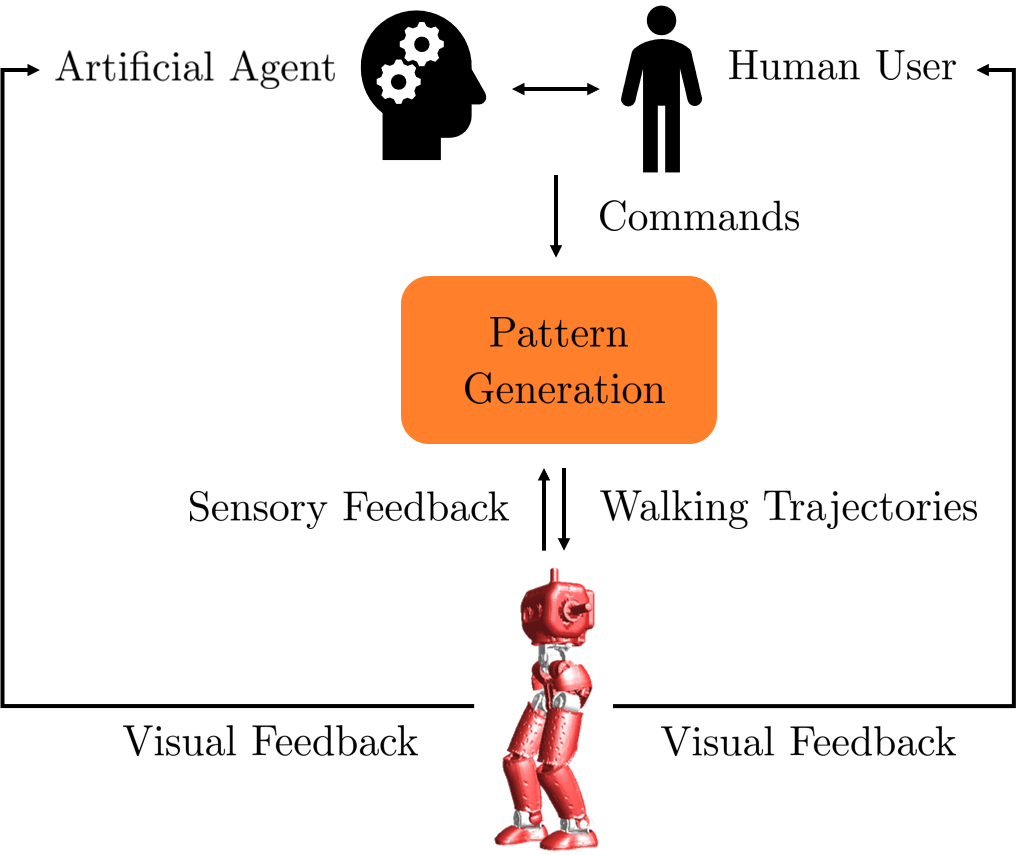
\includegraphics[scale=.5]{chapters/07_autonomous_high_level_control_of_the_walking_pattern_generator/img/control_loop.png}
	\caption{Simplified version of the proposed control loop to navigate the robot with either a human user or an artificial agent. The commands will be given in the form of linear velocities $v_x$, and $v_y$, along the x-, and the y-axis, as well as an angular velocity $\omega_z$ about the z-axis of the robot's coordinates system.}
	\label{fig::2_cl}
\end{figure}
\FloatBarrier
%\label{sec::4_ml}
Machine learning methods do play a major role for autonomous navigation of robots, and whilst most recent approaches mainly dealt with tree search methods in 3D point-clouds, we aim at utilizing neural networks for solving the task at hand, since it enables us to combine spatial, semantic, and temporal understanding into one approach. Within this chapter, we will, therefore, explain the required fundamentals on neural networks in section \ref{sec::41_nn}, then cover two possible methods for training a neural network, one of which is supervised \ref{sec::51_bc}, whereas the second method bases on reinforcement learning \ref{sec::42_rl}, and finally explain image processing techniques in section \ref{sec::3_ip}, which allow us to extract depth maps from stereo images, so to help the neural networks understand the seen content. The goal here clearly is to introduce a method that is biologically inspired, in that it works directly in the image domain, which is very similar to how humans observe their environment. Therefore, we will shortly explain the biological similarities to a human brain within the next section - Neural Networks.
